\section{Rain Sensor Model}
As Fig.4 shows, the rain sensor model is implemented by a FSM. It receives an input, the volume of remaining water, and outputs a control signal to the windshield wiper model. There are 3 states in this FSM. The first state is OFF, when the volume of remaining water is less than 10 ml, the control signal is 0 and the wiper is OFF. The second state is SLOW, when the volume of remaining water is less than 15 ml but exceeds 10 ml, the control signal is 1 and the wiper is SLOW. The third state is FAST, when the volume of remaining water exceeds 15 ml, the control signal is 2 and the wiper is FAST.
\begin{center}
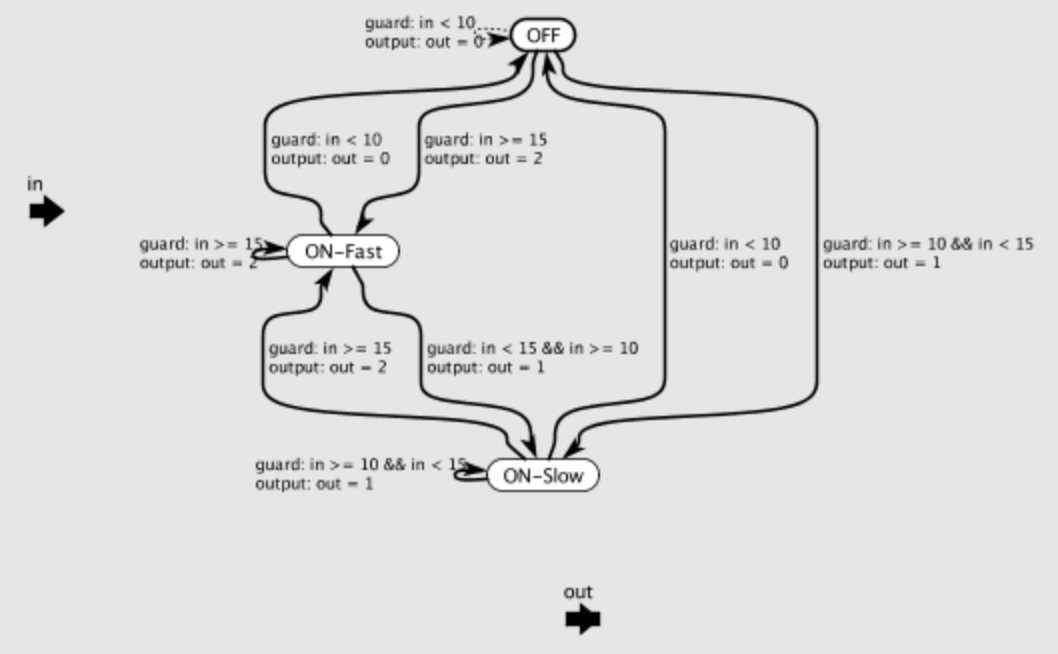
\includegraphics[width=13.5cm]{fig4.png}
\end{center}
\begin{center}
\small{Figure 4. The Rain Sensor Model}
\label{rain_sensor}
\end{center}